\section{FreeRTOS}
\note{Kort intro til hvad FreeRTOS er og hvilken funktionalitet det stiller tilrådighed}
Som indlejret styresystem benyttes FreeRTOS. 
FreeRTOS er et open source real-tids styresystem til indlejrede systemer, som er blevet en industriel standard. 
Styresystemet er valgt, da det er simpelt at gå til. 
Det er desuden primært skrevet i programmeringssproget C, som også benyttes i projektet. 
FreeRTOS benytter preemptive schedulering til at administrere CPU-tiden mellem tasks. 

\section{Preemptive schedulering}
FreeRTOS er bygget på en prioritetsbaseret preemptive scheduleringsalgoritme.\newline
Når et operativ system opererer med en preemptive scheduleringsalgoritme kan kørende processer preemptes - blive stoppet - og skiftet ud med en anden proces.\newline
Det kan f.eks. være at en proces der har ventet på en I/O device får tilgang til denne.
Scheduleren vil så skifte den nuværende kørende proces ud og skifte den hidtil ventende proces ind så den kan køres.
Dette gør scheduleren via et context switch.\newline
Når et context switch sker gemmes ''konteksten`` af den nuværende task i en process control block (PCB), og ydermere sker der et state restore, hvor informationen i PCBen af den task, der skal skiftes til hentes.
Det som bliver gemt i PCBen er værdierne i CPU registrene (Program counter, etc.) og anden vigtig operativ systemsinformation.\newline
Prioritetsbaseret skeduleringsalgoritmer tildeler alle tasks en prioritet som er baseret på taskens vigtighed.\newline
FreeRTOS er et real-time operativ system og et primært formål ved real-time operativ systemer er at give et respons på begivenheder indenfor en vis deadline.
FreeRTOS skeduleringsalgoritme sørger så for at den task med højest prioritet bliver givet processortid.

\section{Interrupt håndtering}
\note{Interrupt execution diagram og opsætning} 
\subsection{Intterrupt eksekvering og task skedulering}
Figur \ref{fig:int_task} viser hvordan tasks og interrupts håndteres i FreeRTOS. 
Til tiden t1 kører en lavt prioriteret task. 
Ved t2 bliver en interrupt service rutine, fremover kaldet en ISR, kaldt. 
Den prioriteres højest, og den lavt prioriteret task pauses indtil ISR'en er færdig.
ISR'eren er færdig til tiden t3, hvor den lavt prioriteret task kan genoptages.
Ved t4 sker et context switch til en højere prioriteret task.
Skeduleringen mellem tasks er styret af FreeRTOS scheduler med respekt til den prioritet, som hver task er givet. 
Interrupts prioriteres højere end alle tasks, uanset prioriteten af den pågældende task. 
Interrupts har også prioriteter i mellem sig, såfremt flere skulle blive kaldt. 
Modsat tasks, vil en interrupt dog altid afsluttes, før den næste kan begynde. 
ARM Cortex-M4 tilbyder otte interrupt prioriteter. 
\husk{Jes}{Forstået rigtigt?} 
\begin{figure}[h]
	\caption{Det tidslige forløb for to tasks og en interrupt service rutine. }
	\centering
	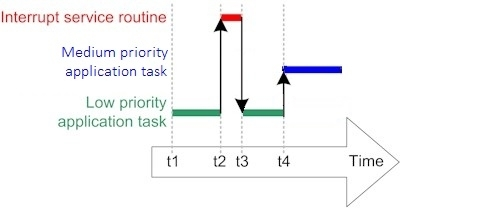
\includegraphics[width=0.7\linewidth]{billeder/interruptandtaskprocessing.jpg}
	\label{fig:int_task}
\end{figure}

Når det indgående lydsignal skal samples gennem ADC'en, skal samplingen foregå periodisk på nøjagtigt det samme tidspunkt i hver periode.
Det faste tidspunkt for sampling giver minimal jitter med en minimal forsinkelse i samplingen af signalet. 
\husk{Jes}{Dansk ord for jitter? Det er et teknisk engelsk ord, så det kan vel gå.. } 
For at sikre, at mikrocontrolleren sætter alle andre opgaver på pause, og begynder at sample på det korrekte tidspunkt, implementeres samplingen i en ISR.

\subsection{Implementering af interrupt-styring med timer}
ISR'en indstilles med den højest mulige interrupt prioritet. 
Timingen af ISR'en er styret af Timer 3. 
Timeren er implementeret som en 16-bit timer i periodic timer mode, edge-count mode og inverted PWM mode.
Ved start hentes timerens start value ind i et tælleregister. 
Sample-frekvensen og CPU frekvensen styrer værdien. 
\begin{equation}
	\text{Timer start value register} = \frac{\text{CPU'ens frekvens}}{\text{Sample-frekvens}} = \frac{80\text{MHz}}{44,1\text{kHz}} \simeq 1814
\end{equation}
I periodic timer mode vil timeren dekrementere fra tælleregisteret, som automatisk henter timer start værdien igen, og begynder forfra når værdien når nul. 
Når værdien når nul, kaldes den ISR som sikrer at lydsignalet bliver samplet. \newline

\subsection{Generering af PWM-signal til DAC}
\husk{Jes}{Hører det til 'Genskabelse af signal via DAC igennem SPI-afsnit'?}
Timeren benyttes desuden til at generere et PWM-signal, hvis duty cycle er styret af timeren og resultatet af A/D konverteringen af indgangssignalet. 
Figur \ref{fig:PWMfromtimer} viser hvordan PWM-signalets duty cycle bliver bestemt af den værdi, som bliver gemt på Timer A's match register. 
Den værdi kommer fra den periodiske sampling af lydsignalet gennem ADC'en, hvor resultatet af hver sampling netop gemmes i match registeret. 
Således genskabes signalet som et digitalt PWM signal. 

% Figur kommer!
% Hvor kommer PWM ud?
% Skal det efter ADC afsnit?

\section{Sampling af lydsignal igennem ADC}

\section{Håndtering af brugergrænseflade og human input interface}

\section{Modulær opbygning af effekter}

\section{Genskabelse af signal via DAC igennem SPI}

